\documentclass[border=10pt]{standalone}
\usepackage{pgfplots}
\pgfplotsset{compat=1.18}
\usetikzlibrary{arrows.meta}

\begin{document}
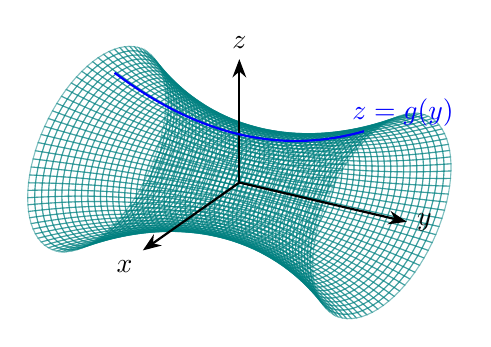
\begin{tikzpicture}
    \begin{axis}[
        axis lines = none,
        view = {120}{35},
        xmin=-2.2, xmax=2.2,
        ymin=-2.4, ymax=2.4,
        zmin=-1.7, zmax=2.2,
        domain = 0:360,
        y domain = -2:2,
        samples = 42,
        samples y = 28,
        ticks=none,
        ]
        % Surface of revolution about the y-axis
        \addplot3[
            surf,
            mesh,
            color = teal,
            faceted color=teal,
            opacity = 0.5,
            domain = 0:360,
            y domain = -2:2,
            samples = 80,
            samples y = 60,
        ] ({(0.82 + 0.18*y^2)*cos(x)}, {y}, {(0.82 + 0.18*y^2)*sin(x)});
        % Positive coordinate axes only
        \draw[-Stealth, thick, black] (axis cs:0,0,0) -- (axis cs:2.15,0,0) node[anchor=north east] {$x$};
        \draw[-Stealth, thick, black] (axis cs:0,0,0) -- (axis cs:0,2.35,0) node[anchor=west] {$y$};
        \draw[-Stealth, thick, black] (axis cs:0,0,0) -- (axis cs:0,0,2.1) node[anchor=south] {$z$};
        % Blue curve z = g(y) (upper generating curve)
        \addplot3[
            blue,
            thick,
            domain = -1.75:1.75,
            samples = 80,
            samples y = 0,
        ] (0, x, {0.82 + 0.18*x^2});
        % Label for the blue curve
        \node[blue, above right] at (axis cs: 0, 1.45, 1.20) {$z = g(y)$};
    \end{axis}
\end{tikzpicture}
\end{document}
